\documentclass{article}

% Hier befinden sich Pakete, die wir beinahe immer benutzen ...

\usepackage[utf8]{inputenc}

% Sprach-Paket:
\usepackage[ngerman]{babel}

% damit's nicht so, wie beim Grill aussieht:
\usepackage{fullpage}

% Mathematik:
\usepackage{amsmath, amssymb, amsfonts, amsthm}
\usepackage{bbm}
\usepackage{mathtools, mathdots}

% Makros mit mehereren Default-Argumenten:
\usepackage{twoopt}

% Anführungszeichen (Makro \Quote{}):
\usepackage{babel}

% if's für Makros:
\usepackage{xifthen}
\usepackage{etoolbox}

% tikz ist kein Zeichenprogramm (doch!):
\usepackage{tikz}

% bessere Aufzählungen:
\usepackage{enumitem}

% (bessere) Umgebung für Bilder:
\usepackage{graphicx, subfig, float}

% Umgebung für Code:
\usepackage{listings}

% Farben:
\usepackage{xcolor}

% Umgebung für "plain text":
\usepackage{verbatim}

% Umgebung für mehrerer Spalten:
\usepackage{multicol}

% "nette" Brüche
\usepackage{nicefrac}

% Spaltentypen verschiedener Dicke
\usepackage{tabularx}
\usepackage{makecell}

% Für Vektoren
\usepackage{esvect}

% (Web-)Links
\usepackage{hyperref}

% Zitieren & Literatur-Verzeichnis
\usepackage[style = authoryear]{biblatex}
\usepackage{csquotes}

% so ähnlich wie mathbb
%\usepackage{mathds}

% Keine Ahnung, was das macht ...
\usepackage{booktabs}
\usepackage{ngerman}
\usepackage{placeins}

% special letters:

\newcommand{\N}{\mathbb{N}}
\newcommand{\Z}{\mathbb{Z}}
\newcommand{\Q}{\mathbb{Q}}
\newcommand{\R}{\mathbb{R}}
\newcommand{\C}{\mathbb{C}}
\newcommand{\K}{\mathbb{K}}
\newcommand{\T}{\mathbb{T}}
\newcommand{\E}{\mathbb{E}}
\newcommand{\V}{\mathbb{V}}
\renewcommand{\S}{\mathbb{S}}
\renewcommand{\P}{\mathbb{P}}
\newcommand{\1}{\mathbbm{1}}

% quantors:

\newcommand{\Forall}{\forall \,}
\newcommand{\Exists}{\exists \,}
\newcommand{\ExistsOnlyOne}{\exists! \,}
\newcommand{\nExists}{\nexists \,}
\newcommand{\ForAlmostAll}{\forall^\infty \,}

% MISC symbols:

\newcommand{\landau}{{\scriptstyle \mathcal{O}}}
\newcommand{\Landau}{\mathcal{O}}


\newcommand{\eps}{\mathrm{eps}}

% graphics in a box:

\newcommandtwoopt
{\includegraphicsboxed}[3][][]
{
  \begin{figure}[!h]
    \begin{boxedin}
      \ifthenelse{\isempty{#1}}
      {
        \begin{center}
          \includegraphics[width = 0.75 \textwidth]{#3}
          \label{fig:#2}
        \end{center}
      }{
        \begin{center}
          \includegraphics[width = 0.75 \textwidth]{#3}
          \caption{#1}
          \label{fig:#2}
        \end{center}
      }
    \end{boxedin}
  \end{figure}
}

% braces:

\newcommand{\pbraces}[1]{{\left  ( #1 \right  )}}
\newcommand{\bbraces}[1]{{\left  [ #1 \right  ]}}
\newcommand{\Bbraces}[1]{{\left \{ #1 \right \}}}
\newcommand{\vbraces}[1]{{\left  | #1 \right  |}}
\newcommand{\Vbraces}[1]{{\left \| #1 \right \|}}
\newcommand{\abraces}[1]{{\left \langle #1 \right \rangle}}
\newcommand{\round}[1]{\bbraces{#1}}

\newcommand
{\floorbraces}[1]
{{\left \lfloor #1 \right \rfloor}}

\newcommand
{\ceilbraces} [1]
{{\left \lceil  #1 \right \rceil }}

% special functions:

\newcommand{\norm}  [2][]{\Vbraces{#2}_{#1}}
\newcommand{\diam}  [2][]{\mathrm{diam}_{#1} \: #2}
\newcommand{\diag}  [1]{\mathrm{diag} \: #1}
\newcommand{\dist}  [1]{\mathrm{dist} \: #1}
\newcommand{\mean}  [1]{\mathrm{mean} \: #1}
\newcommand{\erf}   [1]{\mathrm{erf} \: #1}
\newcommand{\id}    [1]{\mathrm{id} \: #1}
\newcommand{\sgn}   [1]{\mathrm{sgn} \: #1}
\newcommand{\supp}  [1]{\mathrm{supp} \: #1}
\newcommand{\arsinh}[1]{\mathrm{arsinh} \: #1}
\newcommand{\arcosh}[1]{\mathrm{arcosh} \: #1}
\newcommand{\artanh}[1]{\mathrm{artanh} \: #1}
\newcommand{\card}  [1]{\mathrm{card} \: #1}
\newcommand{\Span}  [1]{\mathrm{span} \: #1}
\newcommand{\Aut}   [1]{\mathrm{Aut} \: #1}
\newcommand{\End}   [1]{\mathrm{End} \: #1}
\newcommand{\ggT}   [1]{\mathrm{ggT} \: #1}
\newcommand{\kgV}   [1]{\mathrm{kgV} \: #1}
\newcommand{\ord}   [1]{\mathrm{ord} \: #1}
\newcommand{\grad}  [1]{\mathrm{grad} \: #1}
\newcommand{\ran}   [1]{\mathrm{ran} \: #1}
\newcommand{\graph} [1]{\mathrm{graph} \: #1}
\newcommand{\Inv}   [1]{\mathrm{Inv} \: #1}
\newcommand{\pv}    [1]{\mathrm{pv} \: #1}
\newcommand{\GL}    [1]{\mathrm{GL} \: #1}
\newcommand{\Mod}{\mathrm{Mod} \:}
\newcommand{\Th}{\mathrm{Th} \:}
\newcommand{\Char}{\mathrm{char}}
\newcommand{\At}{\mathrm{At}}
\newcommand{\Ob}{\mathrm{Ob}}
\newcommand{\Hom}{\mathrm{Hom}}
\newcommand{\orthogonal}[3][]{#2 ~\bot_{#1}~ #3}
\newcommand{\Rang}{\mathrm{Rang}}
\newcommand{\NIL}{\mathrm{NIL}}
\newcommand{\Res}{\mathrm{Res}}
\newcommand{\lxor}{\dot \lor}
\newcommand{\Div}{\mathrm{div} \:}
\newcommand{\meas}{\mathrm{meas} \:}

% fractions:

\newcommand{\Frac}[2]{\frac{1}{#1} \pbraces{#2}}
\newcommand{\nfrac}[2]{\nicefrac{#1}{#2}}

% derivatives & integrals:

\newcommandtwoopt
{\Int}[4][][]
{\int_{#1}^{#2} #3 ~\mathrm{d} #4}

\newcommandtwoopt
{\derivative}[3][][]
{
  \frac
  {\mathrm{d}^{#1} #2}
  {\mathrm{d} #3^{#1}}
}

\newcommandtwoopt
{\pderivative}[3][][]
{
  \frac
  {\partial^{#1} #2}
  {\partial #3^{#1}}
}

\newcommand
{\primeprime}
{{\prime \prime}}

\newcommand
{\primeprimeprime}
{{\prime \prime \prime}}

% Text:

\newcommand{\Quote}[1]{\glqq #1\grqq{}}
\newcommand{\Text}[1]{{\text{#1}}}
\newcommand{\fastueberall}{\text{f.ü.}}
\newcommand{\fastsicher}{\text{f.s.}}

% -------------------------------- %
% amsthm-stuff:

\theoremstyle{definition}

% numbered theorems
\newtheorem{theorem}{Satz}
\newtheorem{lemma}{Lemma}
\newtheorem{corollary}{Korollar}
\newtheorem{proposition}{Proposition}
\newtheorem{remark}{Bemerkung}
\newtheorem{definition}{Definition}
\newtheorem{example}{Beispiel}

% unnumbered theorems
\newtheorem*{theorem*}{Satz}
\newtheorem*{lemma*}{Lemma}
\newtheorem*{corollary*}{Korollar}
\newtheorem*{proposition*}{Proposition}
\newtheorem*{remark*}{Bemerkung}
\newtheorem*{definition*}{Definition}
\newtheorem*{example*}{Beispiel}

% Please define this stuff in project ("main.tex"):

% \def \lastexercisenumber {...}
% This will be 0 by default

% \setcounter{section}{...}
% This will be 0 by default
% and hence, completely ignored

\ifnum \thesection = 0
{\newtheorem{exercise}{Aufgabe}}
\else
{\newtheorem{exercise}{Aufgabe}[section]}
\fi

\ifdef
{\lastexercisenumber}
{\setcounter{exercise}{\lastexercisenumber}}

\newcommand{\solution}
{
    \renewcommand{\proofname}{Lösung}
    \renewcommand{\qedsymbol}{}
    \proof
}

\renewcommand{\proofname}{Beweis}

% -------------------------------- %
% environment zum einkasteln:

% dickere vertical lines
\newcolumntype
{x}
[1]
{!{\centering\arraybackslash\vrule width #1}}

% environment selbst (the big cheese)
\newenvironment
{boxedin}
{
  \begin{tabular}
  {
    x{1 pt}
    p{\textwidth}
    x{1 pt}
  }
  \Xhline
  {2 \arrayrulewidth}
}
{
  \\
  \Xhline{2 \arrayrulewidth}
  \end{tabular}
}

% -------------------------------- %
% MISC "Ein-Deutschungen"

\renewcommand
{\figurename}
{Abbildung}

\renewcommand
{\tablename}
{Tabelle}

% -------------------------------- %


\graphicspath{{../../../Fundament-LaTeX/images/}}

\parskip 6 pt
\parindent 0 pt

\title
{
  Logik und Grundlagen der Mathematik \\
  \vspace{4pt}
  \normalsize
  \textit{13. Übung}
}
\author
{
  Richard Weiss
  \and
  Florian Schager
  \and
  Fabian Zehetgruber
}
\date{21.01.2021}

\begin{document}

\maketitle

\section*{Auswahlaxiom, Endlichkeit}

In diesem Abschnitt arbeiten wir mit der Theorie ZF (ohne AC). Die Existenz von
Auswahlfunktionen oder Wohlordnungen dürfen Sie also nur dann verwenden, wenn sie
explizit in der Angabe garantiert wird.

% --------------------------------------------------------------------------------

\begin{exercise}[272]

Betrachten Sie die folgenden Eigenschaften, die eine Menge $A$ haben kann:

\begin{enumerate}[label = \alph*.]
  \item Es gibt eine injektive Abbildung von $\omega$ nach $A$. (\Quote{$\omega \leq A$})
  \item Es gibt eine fast injektive Abbildung von $\omega$ nach $A$.
  (\Quote{fast injektiv}\ bedeutet, dass das Urbild jedes Bildpunktes endlich ist.)
  \item Es gibt eine injektive, aber nicht surjektive Abbildung von $A$ nach $A$.
  \item Es gibt eine fast injektive, aber nicht surjektive Abbildung von $A$ nach $A$.
  \item Für ein (alle) $x \notin A$ gibt es eine Bijektion von $A$ nach $A \cup \Bbraces{x}$.
  (\Quote{$A = A + 1$})
  \item Es gibt eine surjektive, aber nicht injektive Abbildung von $A$ nach $A$.
  \item Es gibt eine surjektive Abbildung von $A$ auf $\omega$. (\Quote{$\omega \leq^* A$})
  \item Es gibt eine surjektive, fast injektive Abbildung von $A$ auf $\omega$.
  \item Es gibt eine injektive Abbildung von $\omega$ nach $P(A)$. (\Quote{$\omega \leq P(A)$})
  \item Es gibt eine injektive Abbildung von $\omega$ in die endlichen Teilmengen von $A$. (\Quote{$\omega \leq P_{fin}(A)$})
  \item Es gibt eine surjektive Abbildung von den endlichen Teilmengen von $A$ auf $\omega$.
  \item $A$ ist unendlich: \Quote{$|A| = \infty$}
  \item Es gibt eine nichtleere Teilmenge von $\mathfrak{P}(A)$ ohne (bez. $\subseteq$) maximales Element.
\end{enumerate}

Geben Sie möglichst viele nichttriviale Implikationen zwischen diesen Aussagen an, die sich in ZF (also ohne Auswahlaxiom) beweisen lassen.

\end{exercise}

% --------------------------------------------------------------------------------

\begin{solution}

Es gilt die Implikationskette: a. $\implies$ b. $\implies$ c. $\implies$ d.

\begin{enumerate}[label = \arabic*.]

  \item Implikation (a. $\implies$ b.):
  
  Klar.

  \item Implikation (b. $\implies$ c.):
  
  \begin{enumerate}[label = \arabic*.]

    \item Lösung:

    Sei $f: \omega \to A$ fast injektiv.
    Wir definieren zuerst die Hilfsfunktion $k: \omega \to \omega$ durch
  
    \begin{align*}
      k(n) = \min \Bbraces{m \in \omega: \forall z < m: f(z) \neq f(m)}.
    \end{align*}
  
    Dann definiere die Funktion $g$ durch
  
    \begin{align*}
      g = \Bbraces{(x, x): x \in A \setminus f(\omega)} \cup \Bbraces{(f(n), f(n+1)): n \in \omega}.
    \end{align*}

    \item Lösung:
    
    Sei $f: \omega \to A$ fast injektiv, d.h.

    \begin{align*}
      \Forall x \in \ran f:
      |f^{-1}[\Bbraces{x}]| < \infty.
    \end{align*}

    Wir fassen $\omega$ und $A$ als Algebren mit leerem Typ auf.
    Auf diese können wir also den Homomorphiesatz anwenden und bekommen eine Abbildung $g$.

    \textbf{Achtung!}
    Möglicherweise braucht der Homomorphiesatz das Auswahlaxiom?
    Anstatt einen beliebigen Repräsentanten $u$ von $U$ zu wählen, kann man in unserem Fall den kleinsten $u := \min U$ (von endlich vielen) wählen, um $g(U) := f(u)$ zu definieren.
    Wir haben es schließlich mit Schuhen und nicht mit Socken zu tun!

    \phantom{}

    \begin{tcolorbox}[standard jigsaw, opacityback = 0]
      \centering
      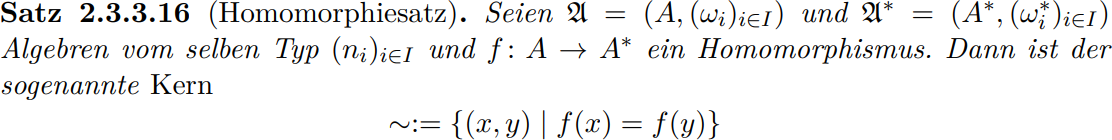
\includegraphics
      [width = 0.75 \textwidth]
      {Alg/Alg - Satz 2.3.3.16.1 (Homomorphiesatz).png} \\
      \vspace{0.25 cm}
      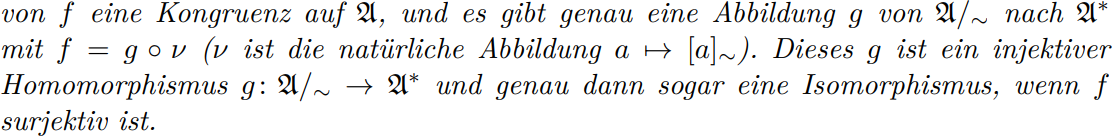
\includegraphics
      [width = 0.75 \textwidth]
      {Alg/Alg - Satz 2.3.3.16.2 (Homomorphiesatz).png} \\
      \vspace{0.25 cm}
      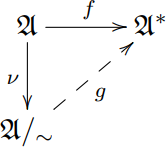
\includegraphics
      [width = 0.15 \textwidth]
      {Alg/Alg - Satz 2.3.3.16.3 (Homomorphiesatz).png}
    \end{tcolorbox}

    \phantom{}

    Seien die (unendlich vielen!) Urbilder gemäß ihrem Minimum, vermöge $h$ (strikt monoton steigend), geordnet, d.h.

    \begin{align*}
      h := (U_n)_{n \in \omega}:
      \omega \to \omega / \sim:
      \min U_1 < \min U_2 < \cdots
    \end{align*}

    $g \circ h: \omega \to A$ ist, als Verkettung injektiver Funktionen, injektiv.

  \end{enumerate}

\end{enumerate}

\end{solution}

% --------------------------------------------------------------------------------


\section*{Zorn, Hausdorff, etc.}

Auch hier arbeiten wir in ZF (ohne AC).

\begin{exercise}
Bestimmen Sie die Momente und die Momentenerzeugende für die Laplaceverteilung
mit der Dichte $f(x) = \frac{1}{2}e^{-|x|}$.
\end{exercise}

\begin{solution}

Trivial

\end{solution}

% -------------------------------------------------------------------------------- %

\begin{exercise}[\textbf{Rolling die}]

A $d$-sided die with colored sides was rolled $n$ times.
The outcomes are stored in the file \texttt{die.Rdata} (each side appeared at least once).

\begin{enumerate}[label = (\alph*)]
    \item Visualize the relative frequencies in a colored barplot and add
    the standard error of each frequency. Given your graphic, what is your
    opinion on the assertion: 'the die is fair'?
    \item Test the null hypothesis that the die is fair with a $\chi^2$-test
    on the 5\%-significance level (without \texttt{chisq.test()})

    \begin{enumerate}[label = \roman*.]
        \item What are the observed (absolute) frequencies?
        What are the expected frequencies under the null hypothesis?
        \item What is the value $x^2$ of the $\chi^2$-statistic?
        How is the $\chi^2$-statistic $X^2$ distributed under the null
        hypothesis (in the context of the associated model).
        \item What is the rejection area? Do you reject the null hypothesis?
        \item Compute the $p$-value and interpret your result.
    \end{enumerate}

    \item Test the null hypothesis that the side 'orange' appears twice as
    often as the other sides (which appear with the same probability),
    on the 10\%-significance level.

    \begin{enumerate}[label = \roman*.]
        \item From the output of \texttt{chisq.test()} read the value
        of the $\chi^2$-statistic and the $p$-value.
        \item Can you reject the null hypothesis?
        \item Based on your calculations someone claims that the die is not
        loaded (i.e., it is fair). What do you answer the person?
    \end{enumerate}
\end{enumerate}

\end{exercise}

% -------------------------------------------------------------------------------- %

\begin{solution}

\phantom{}

\begin{enumerate}[label = (\alph*)]


    \item 

    \begin{figure}[H]
        \centering
        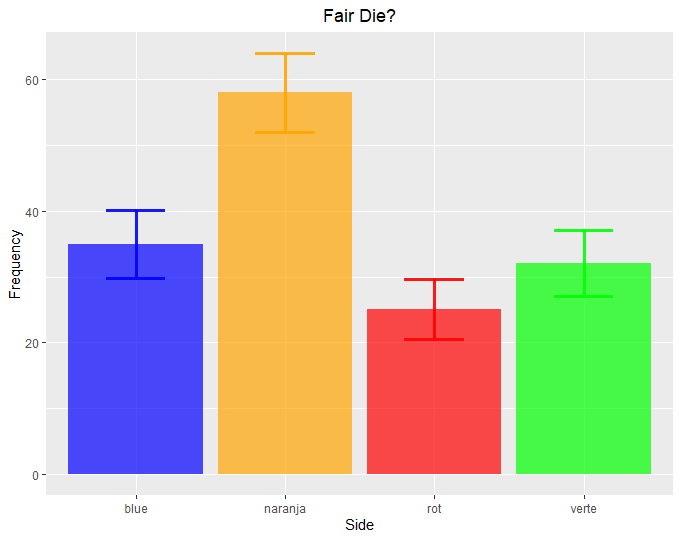
\includegraphics[width = 0.8 \textwidth]{13.3.barplot.png}
    \end{figure}
    Based on the graphical representation of the observed frequencies
    I would guess that the die is biased towards \textit{naranja}.

    \item In our case we have $n = 150$. The observed and expected 
    frequencies under the null are:
    
    \begin{center}
    \begin{tabular}{c|c|c}
        Side & Observed & Expected \\
        \hline
        Blue & 35 & 37.5 \\
        Naranja & 58 & 37.5 \\
        Rot & 25 & 37.5 \\
        Verte & 35 & 37.5
    \end{tabular}
    \end{center}

    Calculating the value of the $X^2$-statistic yields

    \begin{align*}
        X^2 = \frac{2.5^2+20.5^2+12.5^2+2.5^2}{35} \approx 16.83.
    \end{align*}

    Since we know that under the null $X^2 \sim \chi^2(3)$,
    the rejection region at $\alpha = 0.05$ reads

    \begin{align*}
        R = [\chi^2_{\alpha}(3),\infty[ \approx [7.81,\infty[.
    \end{align*}

    Based on the rejection region we reject the null hypothesis that the die is fair.

    Computing the $p$-value yields

    \begin{align*}
        p-\text{value} = \P(X^2 > 16.83) = 0.0007659755 < 0.05,
    \end{align*}

    which agrees with the previous result.

    \item \texttt{chisq.test()} gives the following result:
    
    \begin{lstlisting}
        X-squared = 1.8667, df = 3, p-value = 0.6005
    \end{lstlisting}

    Based on these results we cannot reject the null hypothesis.
    However, this does not conclusively prove the null hypothesis that the die is fair,
    it merely states that there is insufficient evidence to definitively say that the dice is loaded.
\end{enumerate}

\end{solution}

% -------------------------------------------------------------------------------- %

\begin{exercise}
$X$ und $Y$ seien unabhängige Zufallsvariablen.  Zeigen Sie, dass $X + Y$ genau
dann integrierbar ist, wenn $X$ und $Y$ integrierbar sind. (Schätzen Sie in
$\mathbb{E}(Y[|X| < M]),~ |Y|$ mit der Dreiecksungleichung ab; damit kann man
zeigen, dass in der Bedingung für die Existenz von $\mathbb{E}(X)$ der Realteil
von $\phi_X$ durch den Betrag ersetzt werden kann).
\end{exercise}

\begin{solution}

Trivial

\end{solution}

% --------------------------------------------------------------------------------

\begin{exercise}[281]

Sei $A$ eine endliche Menge mit $n$ Elementen. Sei $W(A)$ die Menge aller $(X,R)$,
sodass $X \subseteq A$ ist und $R \subseteq X \times X$ eine lineare Ordnung von $X$
ist. Sei $\simeq$ die Isomorphierelation auf $W(A)$ und $H(A)$ die Menge aller
Äquivalenzklassen.

\begin{enumerate}[label = \alph*.]
  \item Für $A = \{1,2,3\}$: Wie viele Elemente hat $W(A)$? Geben Sie alle an.
  Wie viele Elemente hat $H(A)$? Geben Sie alle an.
  \item Für beliebiges $n$: Wie viele Elemente hat $H(A)$?
\end{enumerate}

\end{exercise}

% --------------------------------------------------------------------------------

\begin{solution}

\phantom{}

\end{solution}

% --------------------------------------------------------------------------------


\section*{Wohlordnungen (2)}

In diesem Abschnitt arbeiten wir mit der Theorie ZF. Die Existenz von Auswahlfunktionen
oder Wohlordnungen dürfen Sie also nur dann verwenden, wenn sie explizit in der Angabe
garantiert wird. \\
Für jede lineare Ordnung $(L,<)$ und $x \in L$ sei $L_x := \{y \in L: y <_L x\}$.
Wir schreiben $A^{<L}$ für die Menge aller Funktionen, deren Definitionsbereich eine
Menge der Form $L_x$ ist, und deren Wertemenge Teilmenge von $A$ ist. \\
Für Wohlordnungen $(X, <)$ und $(Y,<)$ schreiben wir $(X,<) \sqsubset (Y,<)$
(\glqq $X$ ist kürzer als $Y$\grqq), wenn es ein $y_0 \in Y$ gibt mit
$(X, <) \simeq (Y_{<y_0},<)$. Wir schreiben $(X,<) \sqsubseteq$ für
\glqq$(X,<) \sqsubset (Y,<)$ oder $(X,<) \simeq (Y,<)$\grqq.

% --------------------------------------------------------------------------------

\begin{exercise}[286]

Beweisen Sie (in ZFC, informell):
Eine lineare Ordnung $(L, <)$ ist genau dann KEINE Wohlordnung, wenn es eine Funktion $f: \omega \to L$ gibt mit $\Forall n \in \omega: f(n + 1) < f(n)$.
An welchen Stellen Ihres Beweises (wenn überhaupt) verwenden Sie das Auswahlaxiom?

\end{exercise}

% --------------------------------------------------------------------------------

\begin{solution}

Sei $(L, <)$ eine lineare Ordnung.
Zu zeigen ist, dass

\begin{align*}
    (L, <) ~\text{keine Wohlordnung}~
    \iff
    \Exists f: \omega \to L:
        \Forall n \in \omega:
            f(n + 1) < f(n)
\end{align*}

\begin{enumerate}[label = \texttt{ad}]

    \item \Quote{$\implies$}:

    Sei $(L, <)$ keine Wohlordnung, dann

    \begin{align} \label{eq:keine_Wohlordnung}
        \begin{split}
            \Exists E \in \mathcal{P}(L) \setminus \Bbraces{\emptyset}:
                & \nExists l \in E:
                    \Forall l^\prime \in E:
                        l^\prime \leq l \to l = l^\prime \\
                \iff
                & \Forall l \in E:
                    \Exists l^\prime \in E:
                        l^\prime \leq l \land l \neq l^\prime \\
                \stackrel{!}{\iff}
                & \Forall l \in E:
                    \Exists l^\prime \in E:
                        l^\prime < l.
        \end{split}
    \end{align}

    Wir finden jetzt mit dem Auswahlaxiom eine Funktion

    \begin{align*}
        g:
        \mathfrak{P}(L) \setminus \Bbraces{\emptyset} \to L:
            \Forall A \subseteq L:
                g(A) \in A.
    \end{align*}

    Nun definieren wir $E_0 := E$ und $f(0) := g(E_0)$.

    Sei nun $f(n) \in E_{n} := E_{< f(n-1)} \subseteq E$ bereits definiert.
    Weil $f(n) \in E$, gibt es, laut \eqref{eq:keine_Wohlordnung}, ein $f(n + 1) = f(n)^\prime \in E$, sodass $f(n + 1) < f(n)$.
    Also ist $E_{n+1} := E_{<f(n)} \neq \emptyset$ und wir definieren $f(n+1) := g(E_{n+1})$.

    \item \Quote{$\impliedby$}:

    Es gebe eine streng monoton fallende Funktion $f: \omega \to L$.
    Sei $l \in E := f[\omega] \in \mathfrak{P}(L) \setminus \Bbraces{\emptyset}$.

    \begin{align*}
        \implies &
        \Exists n \in \omega:
            l = f(n) > f(n + 1) =: l^\prime \\
        \implies &
        l^\prime \leq l \land l^\prime \neq l
    \end{align*}

    Dafür wird das Auswahlaxiom allerdings nicht gebraucht.

\end{enumerate}

Letzteres \Quote{!} gilt, weil $(L, <)$ ja eine lineare Ordnung ist.

\end{solution}

% --------------------------------------------------------------------------------

% --------------------------------------------------------------------------------

\begin{exercise}[287]

Zeigen Sie (in ZF, ohne AC): Wenn $(A,<)$ eine Wohlordnung ist, dann gibt es eine
lineare Ordnung auf der Potenzmenge von $A$.
\end{exercise}

% --------------------------------------------------------------------------------

\begin{solution}
\textbf{Gescheiterter} erster Versuch: \\
Für alle $B \subseteq A$: Definiere die partielle Funktion $f_B: \omega \to B$ durch
\begin{align*}
  f_B(n) = \begin{cases}
    \min(B \setminus f[\{0,\dots,n-1\}]) & \text{falls }
    B \setminus f[\{0,\dots,n-1\}] \neq \emptyset \\
    \min(A) & \text{sonst}
  \end{cases}
\end{align*}

Wir definieren auf $\mathfrak{P}(A)$
\begin{align*}
  B <_\mathfrak{P} C \iff [\exists n \in \omega: (f_B(n) < f_C(n)) \land \forall k < n: f_B(k) = f_C(k)] \lor (B = \emptyset \land C \neq \emptyset)
\end{align*}

\begin{itemize}
  \item[Irreflexivität:] Klar.
  \item[Transitivität:] Gelte $B <_\mathfrak{P} C$ und $C <_\mathfrak{P} D$. \\
  Dann existieren $n$ und $m$, sodass
  $f_B(n) < f_C(n)$ und $f_C(m) < f_D(m)$. Für $l := \min(n,m)$
  folgt $f_B(l) \leq f_C(l) \leq f_D(l)$, wobei bei mindestens einer Ungleichung
  echt ungleich gelten muss, also $f_B(l) < f_D(l)$ und für alle $k < l: f_B(k) = f_D(k)$.

  \item[Trichotomie:] Gelte $B \nless_\mathfrak{P} C$ und $C \nless_\mathfrak{P} B$
  und $B, C \neq \emptyset$. Also gilt für alle $k \in \N: f_B(k) = f_C(k)$.
  Für endliche Mengen folgt daraus sicher bereits Gleichheit, bei
  unendlichen Mengen könnten vielleicht noch Tricks versteckt sein. \\
\end{itemize}
Problem: Betrachte die Wohlordnung $(\N \cup +\infty, <)$, wobei wir zu den
natürlichen Zahlen ein maximales Element hinzugefügt haben. Dann wären die Mengen
$\N$ und $\N \cup +\infty$ mit unserer linearen Ordnung nicht vergleichbar.




\textbf{Erfolgreicher} zweiter Versuch: \\
Wir definieren $\overline{A} = A \cup \{-\infty\}$ mit $\forall x \in A: -\infty < x$
und weiters $\min(\emptyset) := -\infty$. \\
Auf der Potenzmenge definieren wir

\begin{align*}
  B <_\mathfrak{P} C :\min(B \setminus C) < \min(C \setminus B)
\end{align*}


\begin{center}
\def\r{1}
\def\R{1.3}
\begin{tikzpicture}[scale=1.5]
  \foreach\ang/\name in {-150/b,-30/c,90/d} \draw (\ang:\r) circle (\R) coordinate (\name) node {\name};
  \path (b) -- (c) node [midway] (bc) {bc} ;
  \path (c) -- (d) node [midway] (cd) {cd} ;
  \path (d) -- (b) node [midway] (db) {db} ;
  \path (d) -- (bc) node [pos=.667] (bcd) {bcd};
\end{tikzpicture}
\end{center}

\begin{itemize}
  \item[Irreflexivität:] Klar.
  \item[Transitivität:] Gelte $B <_\mathfrak{P} C$ und $C <_\mathfrak{P} D$. \\
  Wir verwenden ab nun die Kurznotationen aus der Skizze: \\
  (Man beachte, dass die Abkürzungen auch für die leere Menge stehen können)\\
  Laut Voraussetzung gilt also $\min(b \cup db) < \min(c \cup cd)$ und
  $\min(c \cup bc) < \min(d \cup db)$. Damit folgt
  \begin{align*}
    \min(b \cup bc \cup db) = \min(b \cup bc \cup db \cup c \cup cd)
    = \min(b \cup bc \cup db \cup c \cup cd \cup d) \leq \min(d \cup cd)
  \end{align*}
  Angenommen, es gelte $\min(db) < \min(b \cup bc)$, dann erhalten wir mit
  \begin{align*}
  \min(db \cup d) &> \min(c \cup bc) \geq \min(c \cup bc \cup cd) \geq \min(b \cup bc \cup db)
  = \min(db)
  \end{align*}
  einen Widerspruch! Also gilt
  \begin{align*}
    \min(b \cup bc) = \min(b \cup bc \cup db) \leq \min(d \cup cd)
  \end{align*}
  und aufgrund der Disjunktheit gilt sogar die strikte Ungleichung und somit $B <_\mathfrak{P} D$.

  \item[Trichotomie:] Gelte $B \nless_\mathfrak{P} C$ und $C \nless_\mathfrak{P} B$, also
  $\min(B \setminus C) = \min(C \setminus B)$. Dies ist aufgrund der Disjunktheit nur
  möglich, wenn $B \setminus C = C \setminus B = \emptyset$, also $B = C$.
\end{itemize}

\end{solution}

% --------------------------------------------------------------------------------


\section*{Außer Konkurrenz}

\subsection*{288 + 289}

% -------------------------------------------------------------------------------- %

\begin{exercise}[288]

Geben Sei eine explizite Wohlordnung von $V_{\omega}$ an. \\
\textit{Hinweis:} Geben Sie eine explizite Wohlordnung von $V_{n+1} \setminus V_n$ an.
\end{exercise}

% -------------------------------------------------------------------------------- %

\begin{solution}

\phantom{}

\end{solution}

% -------------------------------------------------------------------------------- %

\begin{exercise}[289]

Mit PWW bezeichnen wir den Satz: \glqq Für jede wohlgeordnete Menge $A$ gilt,
dass es auf $\mathfrak{P}(A)$ eine Wohlordnung gibt.\grqq\
Schließen Sie aus ZF+PWW dass es auf $V_{\omega + \omega}$ eine Wohlordnung gibt. \\
\textit{Achtung}: Das ist eine schwierige Aufgabe. Bitte kontrollieren Sie sorgfältig,
ob Sie nicht versehentlich das Auswahlaxiom verwendet haben. Wenn Sie eine einfachen
Beweis gefunden haben, dann ist er ziemlich sicher falsch, weil er nämlich in
versteckter Weise das Auswahlaxiom verwendet.

\end{exercise}

% -------------------------------------------------------------------------------- %

\begin{solution}

\phantom{}

\end{solution}

% -------------------------------------------------------------------------------- %


\end{document}
